
%TC:ignore
\documentclass[a4paper,12pt]{article}
\usepackage[english]{babel}
\usepackage{graphicx}
\usepackage[svgnames, dvipsnames]{xcolor} 
\usepackage{amsmath} 
\usepackage{url}
\usepackage{geometry}
\geometry{margin=1in, right=1.2in} 
\graphicspath{{./}{../images/}} 

\title{My Awesome Document \textit{with Style}}
\author{Dr. LaTeX User}
\date{\today}

\definecolor{mycustomred}{HTML}{CC0000}
\definecolor{mycustomgreen}{rgb}{0,0.5,0}
\newcommand{\important}[1]{\textbf{\textcolor{mycustomred}{#1}}}
\newcommand{\docname}{My Test Doc}
%TC:endignore

\begin{document}

\section{Introduction to \docname}
This is the first paragraph. It includes some \textbf{bold text} and some \textit{italic text}.
Here is a sentence with \important{very important information}.
And now, \textbf{\textit{bold and italic}}! Followed by \underline{underlined text}.
We can also have \texttt{monospace text}. A URL: \url{https://example.com}.
A citation \citep{cox_fish_2023, cox_fish_2023a}. Another one \citep{cox_fish_2023a}.

\subsection{Lists and Things}
An itemized list:
\begin{itemize}
    \item First simple item.
    \item Second item with \textbf{bold parts} and \textit{italic parts}.
    \item A \textcolor{Blue}{blue item}.
    \item {\color{Green}A green item using group syntax}.
\end{itemize}
A numbered list:
\begin{enumerate}
    \item Number one.
    \item Number two, also with \important{emphasis}.
\end{enumerate}

\section{Figures and Tables}
\begin{figure}[h!]
    \centering
    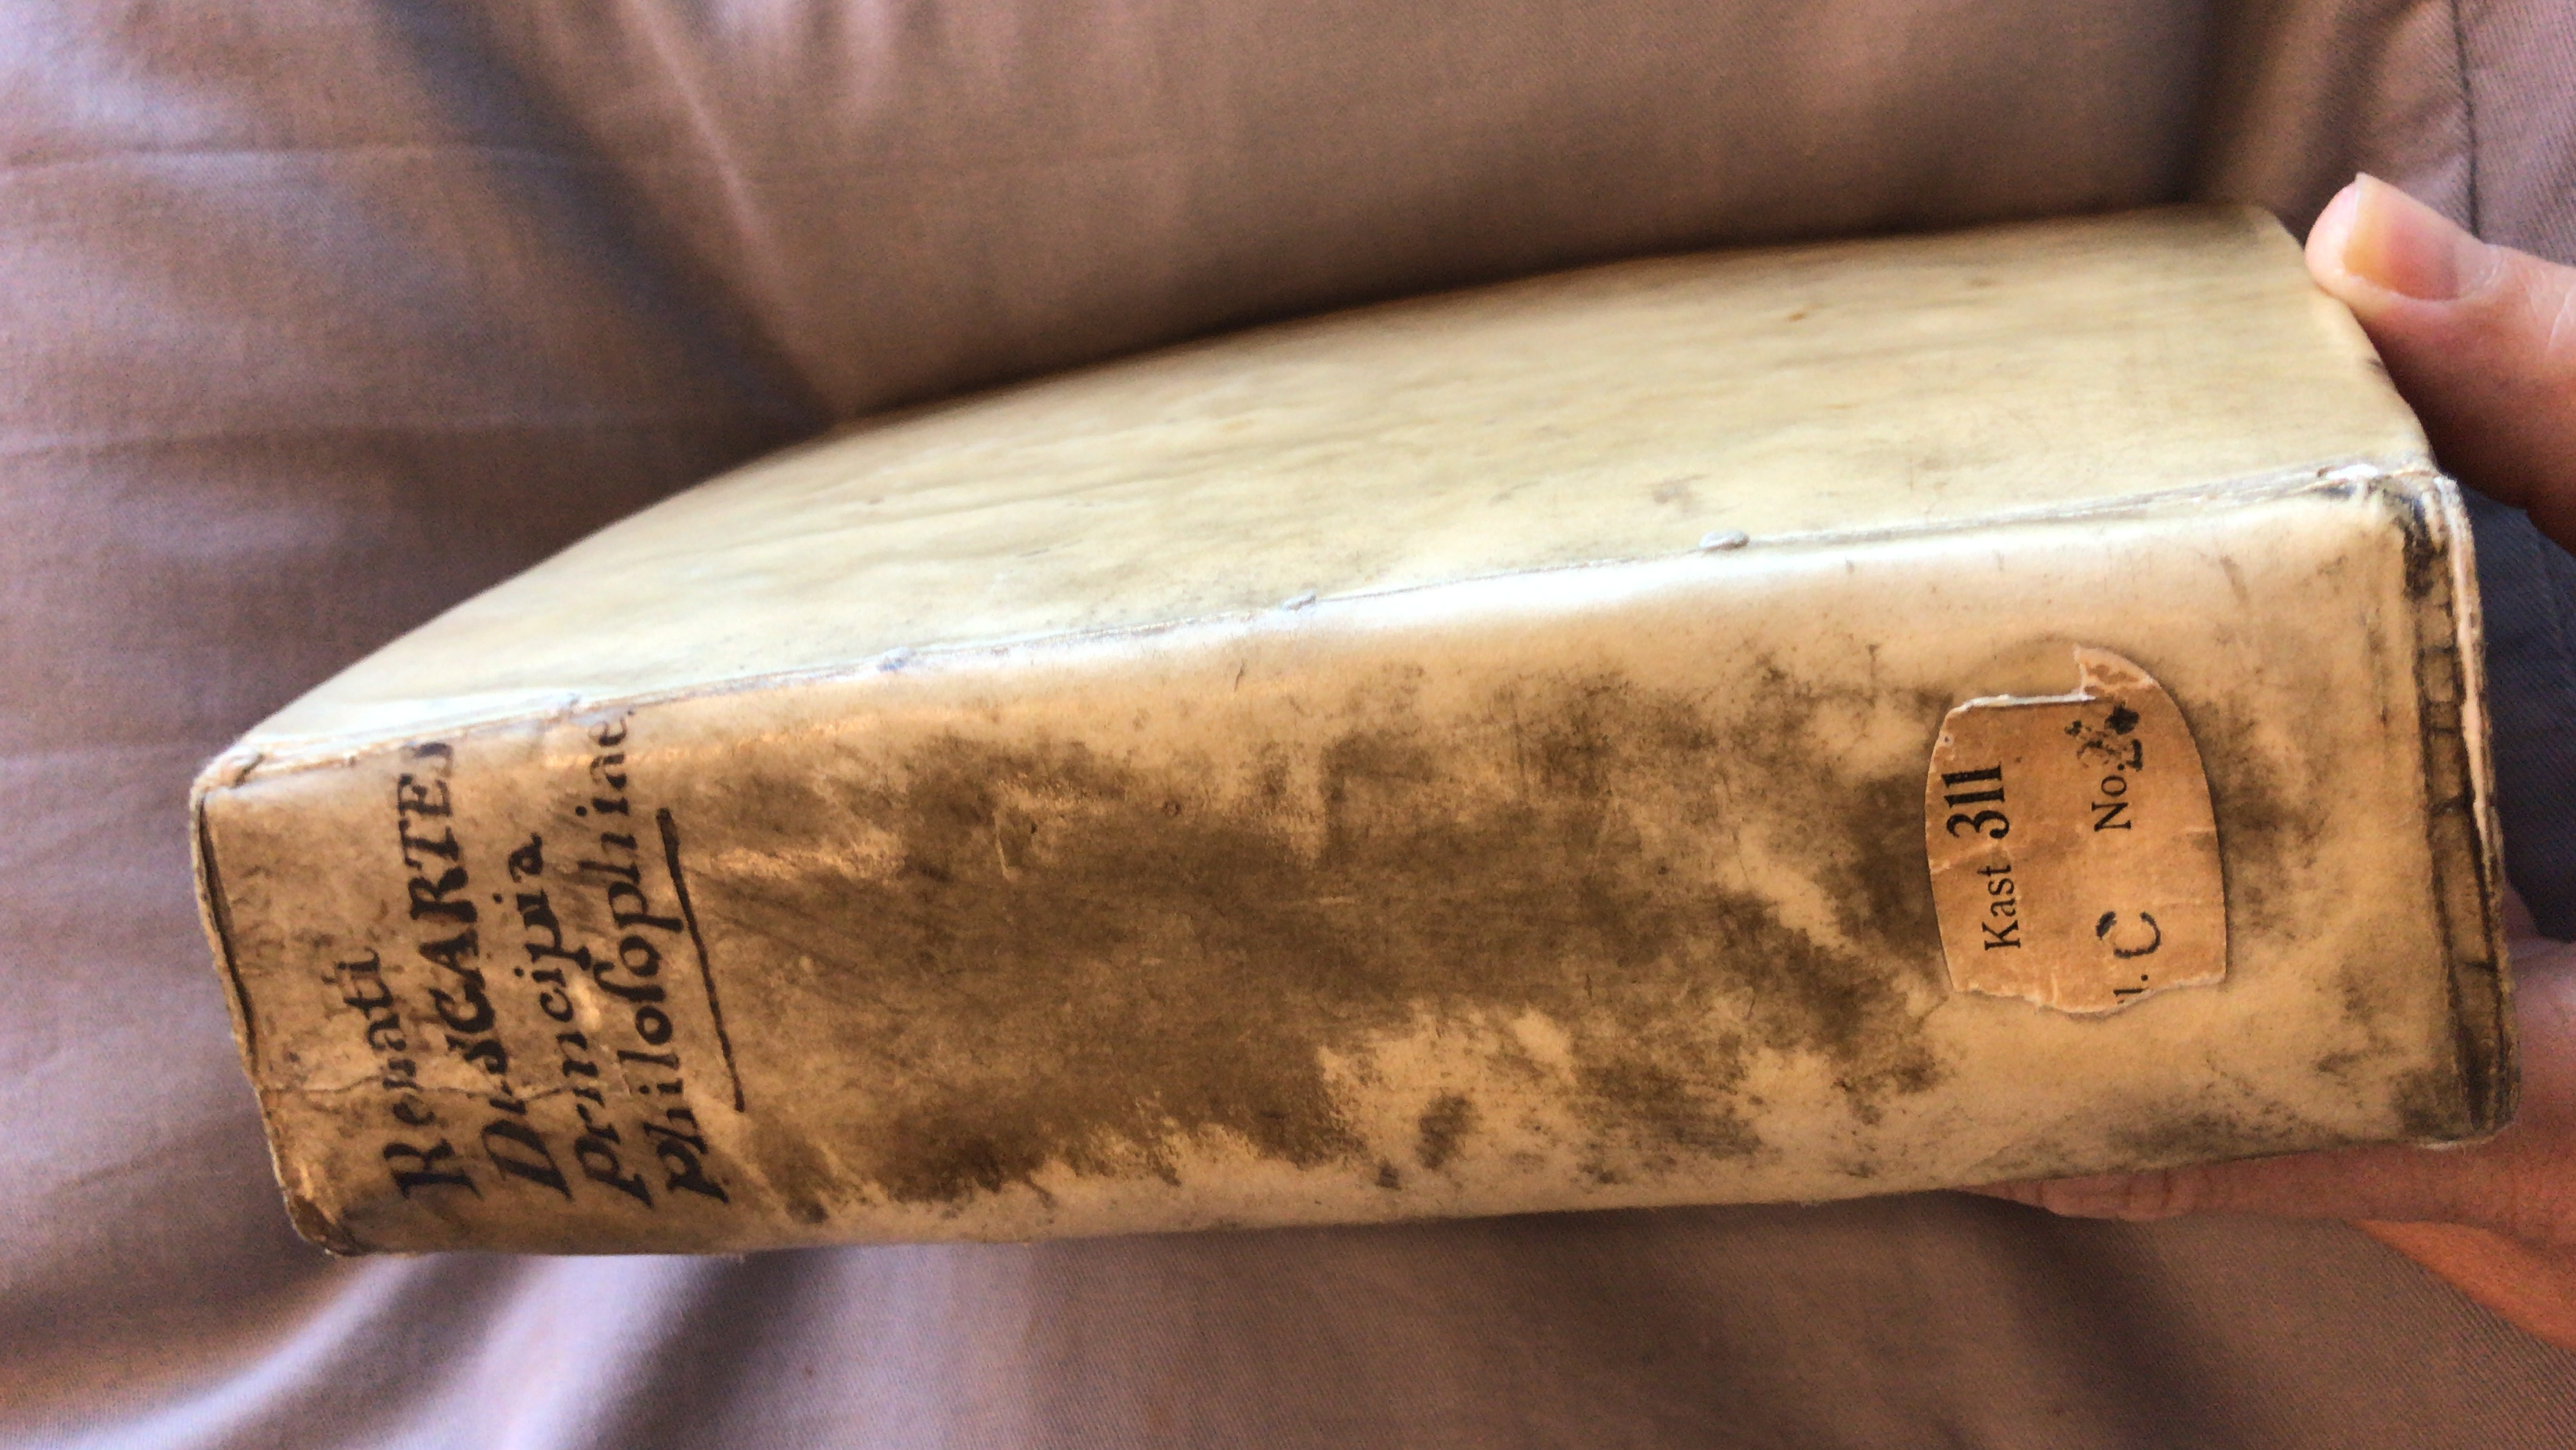
\includegraphics[width=0.5\textwidth, height=5cm]{test.JPG}
    \caption{This is a caption for the example image.}
    \label{fig:example}
\end{figure}

Here is a table:
\begin{tabular}{|l|c|r|}
\hline
Header 1 & Header 2 & Header 3 \\
\hline
Cell 1.1 & Cell 1.2 with \textbf{bold} & Cell 1.3 \\
Cell 2.1 & \textit{Cell 2.2 italic} & Cell 2.3 with \url{https://example.org} \\
\hline
\end{tabular}

\begin{quotation}
This is a quotation environment. It should be indented.
It can also contain \textbf{formatted text}.
\end{quotation}

\newpage
This is after a page break.

\printbibliography 

\end{document}
    